\documentclass{article}

% Language setting
% Replace `english' with e.g. `spanish' to change the document language
\usepackage[english]{babel}

% Set page size and margins
% Replace `letterpaper' with `a4paper' for UK/EU standard size
\usepackage[letterpaper,top=2cm,bottom=2cm,left=3cm,right=3cm,marginparwidth=1.75cm]{geometry}

% Useful packages
\usepackage{amsmath}
\usepackage{graphicx}
\usepackage[colorlinks=true, allcolors=blue]{hyperref}

\title{Aist ass3}
\author{Tsang Cheuk Hang (SID:1155167650}


\begin{document}
\maketitle

\section{Quesiton 1}
\subsection{Why is positional encoding necessary in Transformer models?}

For the model to make use of the order of the sequence, the Transformer model inject some information about the relative or absolute position of the tokens in the sequence. Therefore, the Transformer model add "positional encodings" to the input embeddings at the bottoms of the encoder and decoder stacks. The positional encodings have the same dimension dmodel as the embeddings, so that the two can be summed.

\subsection{Why are sine and cosine functions chosen for positional encoding?}

The sine and cosine functions chosen for positional encoding in Transformer models are because the designers hypothesized that it would allow the model to easialy learn to attend by relative positions, since for any fixed offset $k$, $PE_{pos+k}$ can be represented as a linear function of $PE_{pos}$. Additionally, the authors of the Transformer models also explored using different learned positional embeddings, but the results were nearly the same.

\section{Quesiton 2}
\subsection{(b) Evaluation}
\begin{figure}
    \centering
    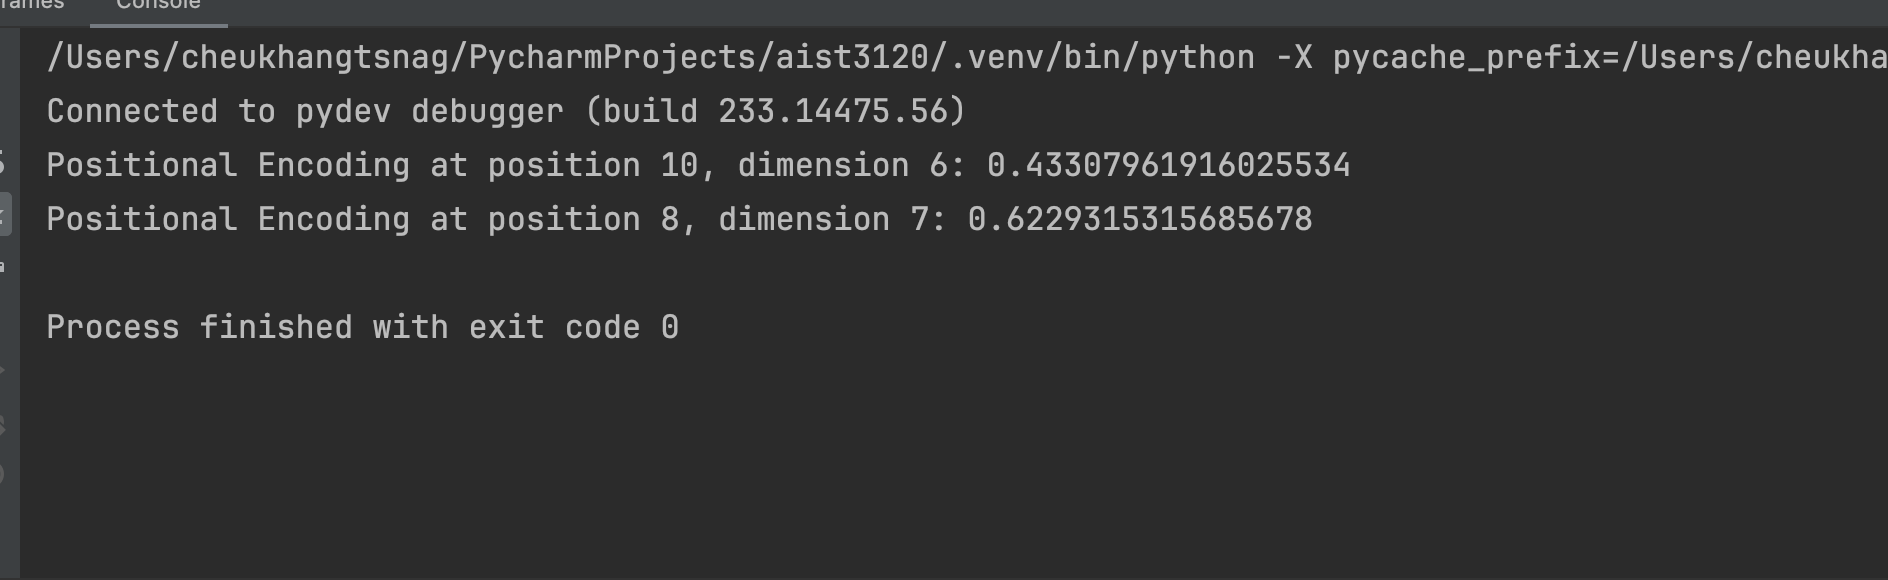
\includegraphics[width=1\linewidth]{image.png}
    \caption{Question 2}
    \label{fig:enter-label}
\end{figure}

\end{document}